\documentclass[t,aspectratio=169]{beamer}
%\usetheme{Berkeley}
\usepackage{graphicx}
\usepackage{amsmath}
\usepackage[american]{circuitikz}

\title{Clase 11}
\subtitle{Reguladores de tensión}
\author{Dr.-Ing. Juan José Montero Rodríguez}
\subject{Elementos Activos}
\institute{Escuela de Ingeniería Electrónica}
\date{Semestre II-2023}

\begin{document}

\begin{frame}{}
\maketitle
\end{frame}

\section{Generalidades}

\begin{frame}{Reguladores de tensión}

En un rectificador, la tensión de salida depende de la tensión de entrada.

\begin{figure}
    \centering
    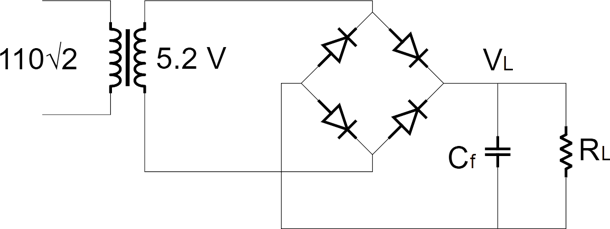
\includegraphics[width=0.5\textwidth]{figures/rectifier.png}
\end{figure}

La tensión de línea de 110 V\textsubscript{RMS} varía durante el día, dependiendo de la carga conectada a la red de distribución.

    \begin{itemize}
        \item La tensión de 5.2 V no es constante.
        \item La tensión de la carga no es constante.
    \end{itemize}

\vspace{5mm}
Además, la tensión de salida contiene un rizo con una frecuencia de 120 Hz.

\end{frame}

\section{Diodos de silicio}

\begin{frame}{Regulador con diodo de silicio}

\begin{columns}
\begin{column}{0.5\textwidth}
    Considere el siguiente circuito:
    
    \vspace{5mm}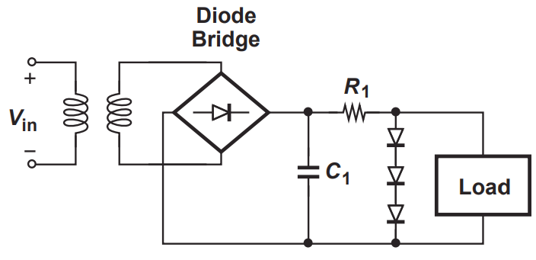
\includegraphics[width=\textwidth]{figures/rectifier_with_regulator.png}
\end{column}
\begin{column}{0.5\textwidth}
    Los tres diodos en serie mantienen la tensión de salida fija:

    \[ V_D = 0.7\ V \]
    \[ V_{out} = 3 V_D = 2.1\ V \]

    \vspace{5mm}La tensión en la resistencia R1 es:

    \[ V_{R1} = V_{C1} - 3V_D  \]
\end{column}
\end{columns}

\vspace{5mm}Esta configuración provee tensiones de salida constantes.

\begin{itemize}
    \item Si $V_{C1}$ aumenta, $V_{R1}$ aumenta, $V_{out}$ permanece constante.
    \item Si $V_{C1}$ disminuye, $V_{R1}$ disminuye, $V_{out}$ permanece constante.
\end{itemize}

\end{frame}


\begin{frame}{Ejemplo 1: Regulador con diodo de silicio}

En el circuito de la figura se desea obtener una tensión de salida de 0.7 V utilizando un diodo de silicio con $I_S = 10^{-14}\ A$. La resistencia $R_S = 100\ \Omega$.

\begin{figure}
    \centering
    \begin{circuitikz}
        \draw (0,2) to [V,l=$V_S$,a=$12\ V$] (0,0);
        \draw (0,2) to [R,l=$R_S$] (3,2);
        \draw (3,2) to [D,l=$V_D$] (3,0);
        \draw (3,2) -- (5,2);
        \draw (5,2) to [R,l=$R_L$] (5,0);
        \draw (0,0) -- (5,0);
    \end{circuitikz}
\end{figure}

Calcule de manera exacta la tensión de salida si el circuito opera:

\begin{enumerate}
    \item Sin carga conectada.
    \item Con una carga $R_L=1000\ \Omega$.
    \item Con una carga $R_L=10\ \Omega$.
\end{enumerate}
    
\end{frame}


\begin{frame}{Solución 1: Regulador con diodo de silicio}

\begin{columns}
\begin{column}{0.5\textwidth}
1. Sin carga conectada:
%
\[ V_S = V_R + V_D \]
%
\[ V_S = I_D R_S + V_t \ln \left( \dfrac{I_D}{I_S} \right) \]
%
\[ 12\ V = I_D\cdot{}100\ \Omega + 26\ mV\cdot{} \ln \left( \dfrac{I_D}{10^{-14}\ A} \right) \]
%
\[ I_D = 112.187\ mA \]
%
\[ V_D = V_t \ln \dfrac{I_D}{I_S} = 26\ mV\cdot{}\ln{}\left( \dfrac{112.187\ mA}{10^{-14}\ A} \right) \]
%
\[ V_D = 781.26\ mV \]
\end{column}
\begin{column}{0.5\textwidth}
    \begin{figure}
    \centering
    \begin{circuitikz}
        \draw (0,2) to [V,l=$V_S$,a=$12\ V$] (0,0);
        \draw (0,2) to [R,l=$R_S$] (3,2);
        \draw (3,2) to [D,l=$V_D$] (3,0);
        \draw (3,2) -- (5,2);
        \draw (5,2) to [R,l=$R_L$] (5,0);
        \draw (0,0) -- (5,0);
    \end{circuitikz}
\end{figure}
\end{column}
\end{columns}
\end{frame}


\begin{frame}{Solución 1: Regulador con diodo de silicio}

\begin{columns}
\begin{column}{0.5\textwidth}
2. Con una carga de $1000\ \Omega$:
%
\[ I_{RS} = I_D + I_{RL} \]
%
\[ \dfrac{V_S - V_D}{R_S} = I_D + \dfrac{V_D}{R_L} \]
%
\[ \dfrac{V_S - V_t \ln (I_D/I_S)}{R_S} = I_D + \dfrac{V_t \ln (I_D/I_S)}{R_L} \]
%
Resolviendo esta ecuación para $I_D$:
%
\[ I_D = 111.408\ mA \]
%
\[ V_D = V_t \ln \dfrac{I_D}{I_S} = 26\ mV\cdot{}\ln{}\left( \dfrac{111.408\ mA}{10^{-14}\ A} \right) \]
%
\[ V_D = 781.08\ mV \]
\end{column}
\begin{column}{0.5\textwidth}
    \begin{figure}
    \centering
    \begin{circuitikz}
        \draw (0,2) to [V,l=$V_S$,a=$12\ V$] (0,0);
        \draw (0,2) to [R,l=$R_S$] (3,2);
        \draw (3,2) to [D,l=$V_D$] (3,0);
        \draw (3,2) -- (5,2);
        \draw (5,2) to [R,l=$R_L$] (5,0);
        \draw (0,0) -- (5,0);
    \end{circuitikz}
\end{figure}
\end{column}
\end{columns}
\end{frame}


\begin{frame}{Solución 1: Regulador con diodo de silicio}

\begin{columns}
\begin{column}{0.5\textwidth}
3. Con una carga de $10\ \Omega$:
%
\[ I_{RS} = I_D + I_{RL} \]
%
\[ \dfrac{V_S - V_D}{R_S} = I_D + \dfrac{V_D}{R_L} \]
%
\[ \dfrac{V_S - V_t \ln (I_D/I_S)}{R_S} = I_D + \dfrac{V_t \ln (I_D/I_S)}{R_L} \]
%
Resolviendo esta ecuación para $I_D$:
%
\[ I_D = 37.217\ mA \]
%
\[ V_D = V_t \ln \dfrac{I_D}{I_S} = 26\ mV\cdot{}\ln{}\left( \dfrac{37.217\ mA}{10^{-14}\ A} \right) \]
%
\[ V_D = 752.58\ mV \]
\end{column}
\begin{column}{0.5\textwidth}
    \begin{figure}
    \centering
    \begin{circuitikz}
        \draw (0,2) to [V,l=$V_S$,a=$12\ V$] (0,0);
        \draw (0,2) to [R,l=$R_S$] (3,2);
        \draw (3,2) to [D,l=$V_D$] (3,0);
        \draw (3,2) -- (5,2);
        \draw (5,2) to [R,l=$R_L$] (5,0);
        \draw (0,0) -- (5,0);
    \end{circuitikz}
\end{figure}
\end{column}
\end{columns}
\end{frame}


\begin{frame}{El modelo de pequeña señal}
    Si se aplica una tensión alterna a un diodo:

    \[ V_D(t) = V_p \sin(\omega t + \phi) \]
    
    La corriente que se obtiene es:

    \[ I_D(t) = I_S \cdot e^{\dfrac{V_D(t)}{V_t}} =  I_S \cdot e^{\dfrac{ V_p \sin(\omega t + \phi) }{V_t}}  \]

    La tensión se puede expresar en forma fasorial, pero la corriente no.

    \begin{block}{Modelo de pequeña señal}
    Si la señal aplicada $V_D$ es pequeña, existe un método para linealizar la corriente, denominado el \textbf{modelo de pequeña señal}. Consiste en aproximar la ecuación exponencial por una ecuación lineal en el punto de operación. 
    \end{block}
\end{frame}


\begin{frame}{Modelo de pequeña señal por derivada}
\begin{columns}
\begin{column}{0.5\textwidth}
    Al aplicar una tensión CD y una variación de tensión CA a un diodo, se obtiene la siguiente forma de onda para la corriente:
    
    \begin{figure}
        \centering
        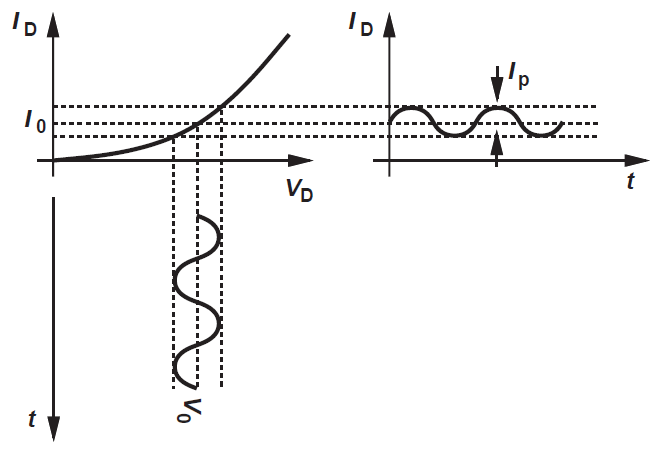
\includegraphics[width=\textwidth]{figures/diode_small_signal.png}
    \end{figure}
\end{column}
\begin{column}{0.5\textwidth}
    La corriente en el diodo es:
    %
    \[ I_D(t) = I_S e^{V_D(t)/V_t} \]
    %
    Se define la \textbf{transconductancia} como derivada de la corriente en el punto de operación:
    %
    \[ g_m = \left. \dfrac{dI_D(t)}{dt} \right|_Q \]
    %
    \[ g_m = \dfrac{I_S}{V_t} e^{V_D(t)/V_t} \]
    %
    \[ g_m = \dfrac{I_{DQ}}{V_t} \]
\end{column}
\end{columns}
\end{frame}


\begin{frame}{Modelo de pequeña señal por serie de Taylor}
\begin{columns}
\begin{column}{0.5\textwidth}
    Al aplicar una tensión de CD y una tensión de CA de manera simultánea, se obtiene:
    %
    \[ i_D(t) = I_S \cdot e^{(V_D+v_d(t))/V_t} \]
    %
    \[ i_D(t) = I_S \cdot e^{V_D/V_t} \cdot e^{v_d(t)/V_t} \]
    %
    La expansión en serie de Taylor:
    %
    \[ i_D(t) = I_{DQ} \left( 1 + x + \dfrac{x^2}{2!} + \dfrac{x^3}{3!} + ... \right) \]
    %
    Donde $x = v_d(t)/V_t$.
\end{column}
\begin{column}{0.5\textwidth}
    Tomando sólo los primeros dos términos (parte lineal):
    %
    \[ i_D(t) = I_{DQ} \left(1 + \dfrac{v_d(t)}{V_t}\right) \]
    %
    \[ i_D(t) = I_{DQ} + \dfrac{I_{DQ}}{V_t} v_d(t) \]
    %
    \[ i_D(t) = I_{DQ} + g_m \cdot v_d(t) \]
    %
    La corriente se compone del valor CD y de una componente de CA que depende de la transconductancia.
\end{column}
\end{columns}
\end{frame}


\begin{frame}{Ejemplo 2: Disminución del rizo}
Considere el circuito rectificador de onda completa de la figura:

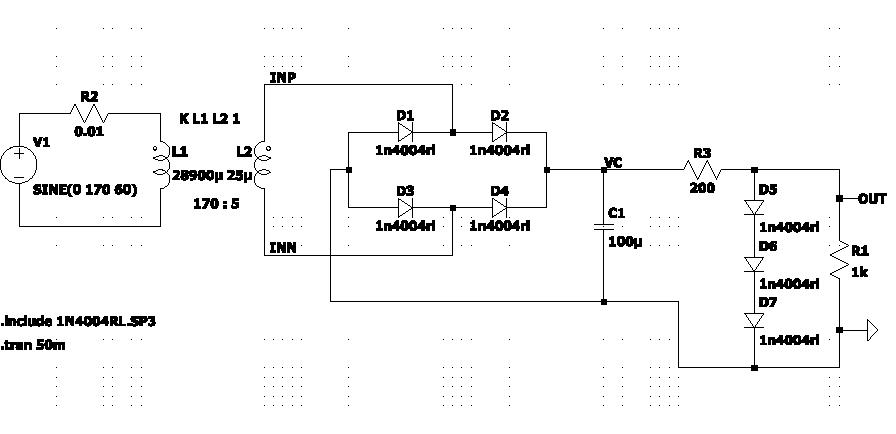
\includegraphics[width=0.8\textwidth]{figures/fullwave_rectifier_schematic.pdf}

\begin{enumerate}
    \item Calcule el valor de la tensión de rizo sin el regulador de diodos.
    \item Determine el valor de la tensión de rizo de salida después de conectar el regulador.
\end{enumerate}

\end{frame}


\begin{frame}{Solución 2: Simulación del rizo}
\begin{columns}
\begin{column}{0.6\textwidth}
    \begin{figure}
        \centering
        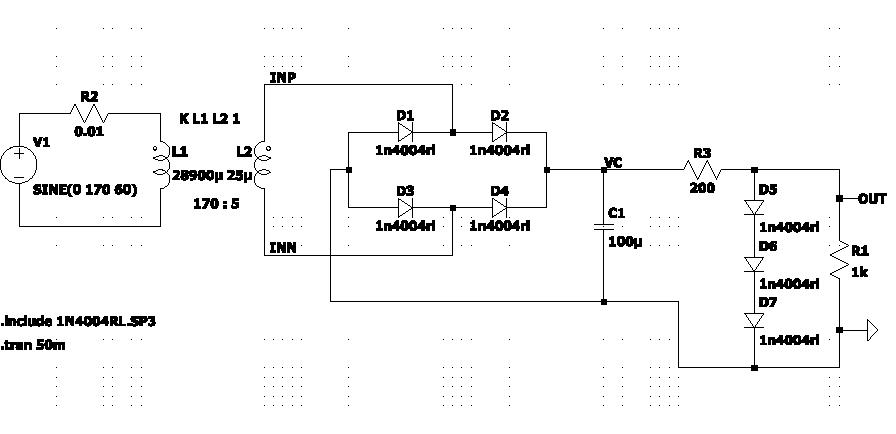
\includegraphics[width=\textwidth]{figures/fullwave_rectifier_schematic.pdf}
    \end{figure}
    %
    \[ I_{L} = \dfrac{5\ V - 2\times{}0.7\ V}{R_L} = \dfrac{3.6\ V}{1\ k\Omega} = 3.6\ mA \]
    %
    \[ V_r = \dfrac{I_L T}{2 C_f} = \dfrac{(3.6\ mA)(1/60 Hz)}{2 (100\ \mu F)} = 300\ mV \]
\end{column}
\begin{column}{0.4\textwidth}
\begin{figure}
    \centering
    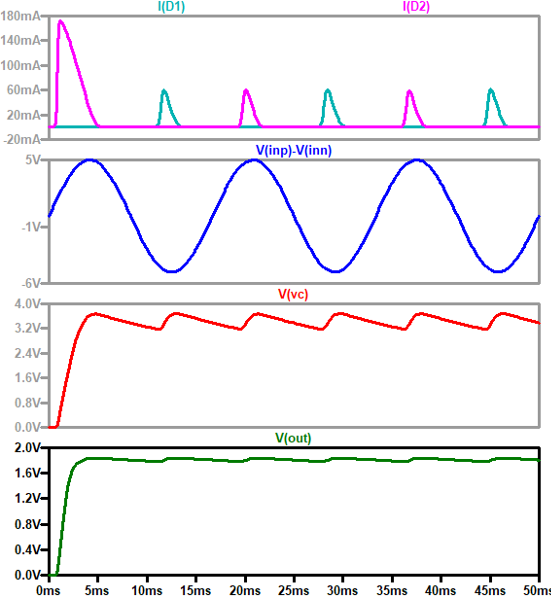
\includegraphics[width=\textwidth]{figures/fullwave_rectifier_ripple_regulation.png}
\end{figure}
\end{column}
\end{columns}
\end{frame}



\begin{frame}{Solución 2: Simulación del rizo}
\begin{columns}
\begin{column}{0.6\textwidth}
    \begin{figure}
        \centering
        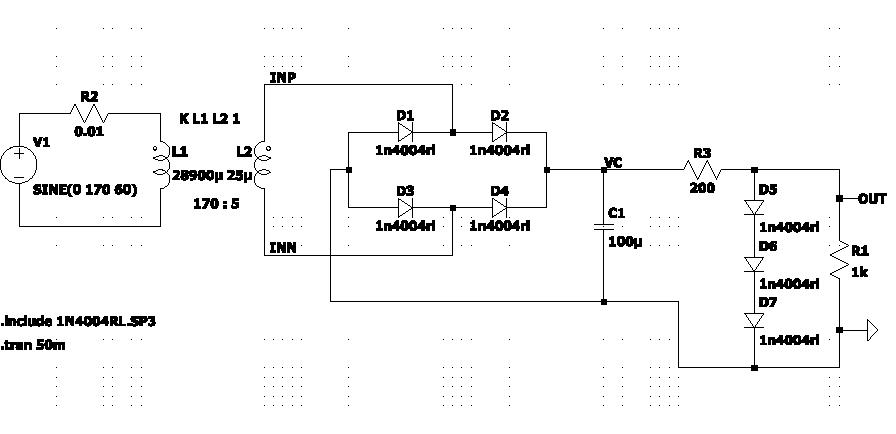
\includegraphics[width=\textwidth]{figures/fullwave_rectifier_schematic.pdf}
    \end{figure}
    %
    \[ r_d = \dfrac{1}{g_m} = \dfrac{V_t}{I_{DQ}} = \dfrac{26\ mV}{5.4\ mA} = 4.81\ \Omega \]
    %
    \[ \Delta V_L = \dfrac{V_r \times 3 r_d}{R_3 + 3 r_d} = 20.19\ mV \]
\end{column}
\begin{column}{0.4\textwidth}
\begin{figure}
    \centering
    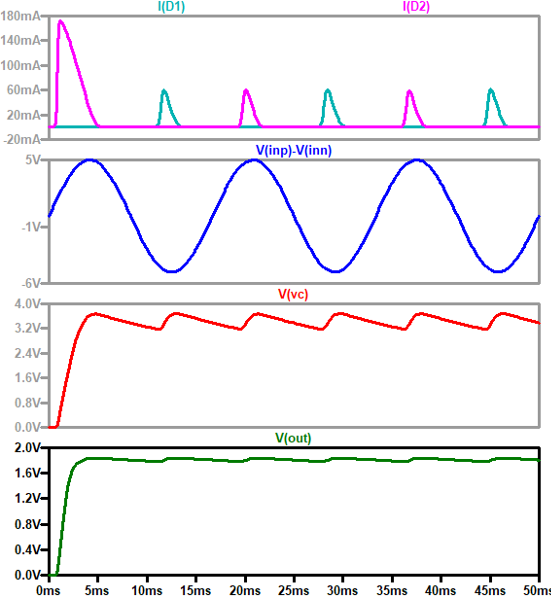
\includegraphics[width=\textwidth]{figures/fullwave_rectifier_ripple_regulation.png}
\end{figure}
\end{column}
\end{columns}
\end{frame}

\section{Diodo Zener}

\begin{frame}{El diodo Zener}


\begin{columns}
\begin{column}{0.6\textwidth}
    El diodo Zener tiene una tensión de reversa constante cuando se conecta con la siguiente polaridad:

    \begin{figure}
        \centering
        \begin{circuitikz}
            \draw (0,0) to [zzDo,a=$V_Z$] (2,0);
            \draw (0.25,-0.25) node [] {$-$};
            \draw (1.75,-0.25) node [] {$+$};
        \end{circuitikz}
    \end{figure}
    
    Existen diodos Zener de distintas tensiones, por ejemplo $V_Z = 3.6\ V$ o $V_Z = 5.1\ V$.

    \vspace{5mm}La corriente nominal de un diodo Zener es $I_{ZT}$.

    \vspace{5mm}La tensión de directa es similar a la de un diodo de silicio, entre 0.3 y 0.7 V.
    
\end{column}
\begin{column}{0.4\textwidth}
\begin{figure}
    \centering
    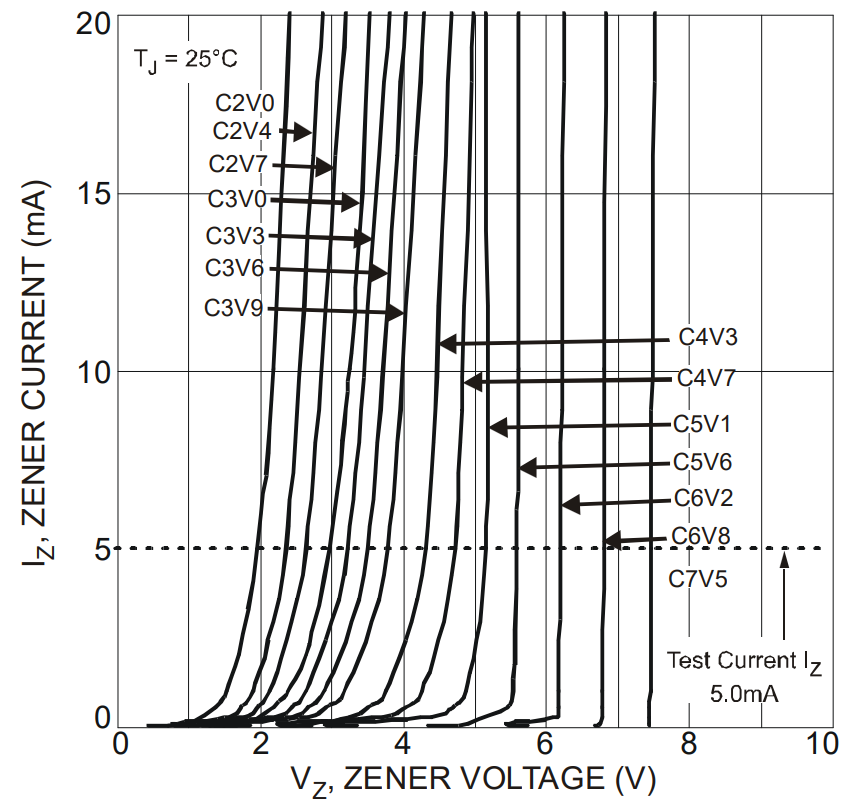
\includegraphics[width=\textwidth]{figures/zener_curves.png}
\end{figure}    
\end{column}
\end{columns}

\end{frame}


\begin{frame}{Regulador con diodo Zener}

\begin{columns}
\begin{column}{0.5\textwidth}
    Considere el siguiente circuito:
    
    \vspace{5mm}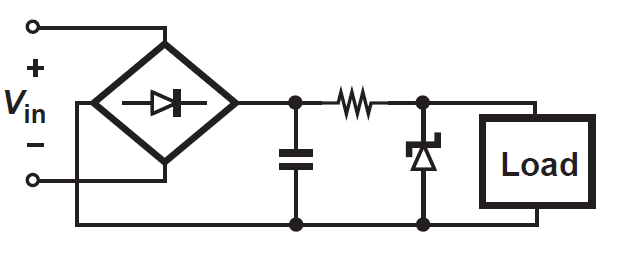
\includegraphics[width=\textwidth]{figures/rectifier_with_zener.png}
\end{column}
\begin{column}{0.5\textwidth}
    \[ I_R = \dfrac{V_C - V_Z}{R_S} \]
    \[ I_L = \dfrac{V_Z}{R_L} \]
    \[ I_Z = I_R - I_L \]
\end{column}
\end{columns}

\vspace{5mm}El diodo Zener mantiene la tensión de salida relativamente constante, siempre y cuando opere con corriente nominal $I_Z = I_{ZT}$.

\begin{itemize}
    \item Si la tensión del condensador aumenta, la corriente por el Zener aumenta.
    \item Si la corriente de la carga aumenta, la corriente por el Zener disminuye.
\end{itemize}
\end{frame}

\begin{frame}{Regulación de línea y regulación de carga}

\begin{itemize}
    \item La tensión $V_Z = 3.6\ V$ sólo es válida si la corriente es nominal $I_{ZT} = 5\ mA$.
    \item Si la fuente $V_S$ cambia, o varía la carga $R_L$, la corriente $I_Z$ es distinta.
    \item Si la corriente $I_Z$ cambia, la tensión $V_Z$ cambia.
\end{itemize}

\vspace{5mm}
\begin{columns}
    \begin{column}{0.5\textwidth}
        La regulación de línea se define como:

        \[ LineReg = \dfrac{V_{out,max} - V_{out,min}}{V_{in,max} - V_{in,min}} \times 100\% \]
        
        Suponiendo que la tensión de entrada de un circuito varía $\pm{}10\%$, se puede resolver el circuito para determinar la variación en la tensión de salida.
    \end{column}
    \begin{column}{0.5\textwidth}
        La regulación de carga se define como:

        \[ LoadReg = \dfrac{V_{out,RLmin} - V_{out,RLmax}}{V_{out,RLnominal}} \times 100\% \]

        Suponiendo que la carga RL varía un $\pm{}10\%$, se puede resolver el circuito para determinar la variación en la tensión de salida.
    \end{column}
\end{columns}
\end{frame}


\begin{frame}{Ejemplo 3: Regulador con diodo Zener}
\begin{itemize}
    \item Diseñe un circuito regulador de tensión con diodo Zener. Este circuito debe convertir una tensión de entrada $V_S = 12\ V$ a una tensión de salida $V_{out} = 3.6\ V$.
    \item El diodo es un Zener modelo BZT52C3V6, fabricado por Diodes Inc. [1], el cual tiene una corriente nominal $I_{ZT} = 5\ mA$ y una tensión Zener $V_Z = 3.6\ V$.
    \item El regulador debe suministrar una tensión constante a una resistencia de carga $R_L$ con un valor nominal de 1000 $\Omega$.
\end{itemize}

\begin{figure}
    \centering
    \begin{circuitikz}
        \draw (0,2) to [V,l=$V_S$,a=$12\ V$] (0,0);
        \draw (0,2) to [R,l=$R_S$] (3,2);
        \draw (3,0) to [zzDo,l_=$V_Z$] (3,2);
        \draw (3,2) -- (5,2);
        \draw (5,2) to [R,l=$R_L$] (5,0);
        \draw (0,0) -- (5,0);
    \end{circuitikz}
\end{figure}
\end{frame}


\begin{frame}{Solución 3: Cálculos}

\begin{figure}
    \centering
    \begin{circuitikz}
        \draw (0,2) to [V,l=$V_S$,a=$12\ V$] (0,0);
        \draw (0,2) to [R,l=$R_S$] (3,2);
        \draw (3,0) to [zzDo,l_=$V_Z$] (3,2);
        \draw (3,2) -- (5,2);
        \draw (5,2) to [R,l=$R_L$] (5,0);
        \draw (0,0) -- (5,0);
    \end{circuitikz}
\end{figure}

\[ I_{RL} = \dfrac{V_Z}{R_L} = \dfrac{3.6\ V}{1000\ \Omega} = 3.6\ mA \]
\[ R_S = \dfrac{V_{RS}}{I_{RS}} = \dfrac{V_S - V_Z}{I_Z + I_L} = \dfrac{12\ V - 3.6\ V}{5\ mA + 3.6\ mA} = 976.74\ \Omega \]
\end{frame}


\begin{frame}{Solución 3: Punto de operación}

\begin{columns}
\begin{column}{0.5\textwidth}
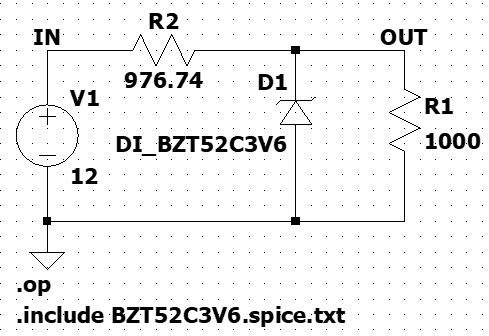
\includegraphics[width=\textwidth]{figures/zener_reg_op.png}
\end{column}
\begin{column}{0.5\textwidth}
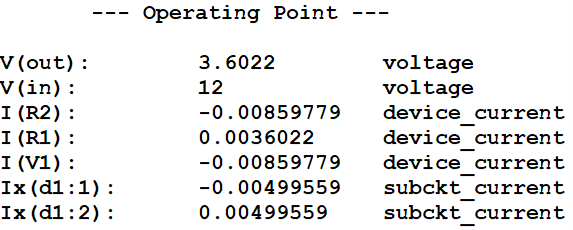
\includegraphics[width=\textwidth]{figures/zener_reg_op2.png}
\end{column}
\end{columns}

\end{frame}


\begin{frame}{Solución 3: Regulación de línea}

\begin{columns}
\begin{column}{0.4\textwidth}
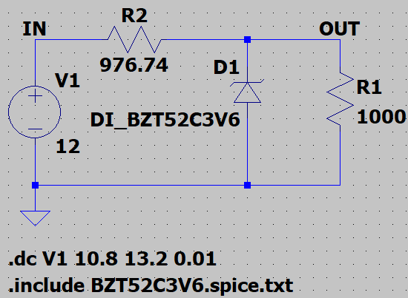
\includegraphics[width=\textwidth]{figures/linereg_schem.png}
\end{column}
\begin{column}{0.3\textwidth}
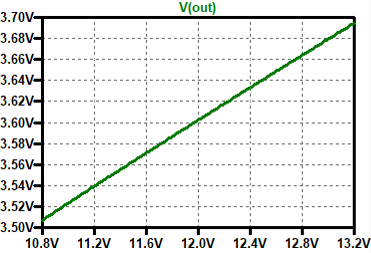
\includegraphics[width=\textwidth]{figures/linereg_plot.png}
\end{column}
\begin{column}{0.3\textwidth}
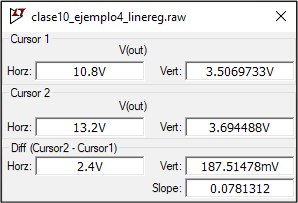
\includegraphics[width=\textwidth]{figures/linereg_measure.png}
\end{column}
\end{columns}

\[ LineReg = \dfrac{3.694488 - 3.5069733}{13.2 - 10.8} \times 100\% \]
\[ LineReg = 7.81\% \]
\end{frame}


\begin{frame}{Solución 3: Regulación de carga}

\begin{columns}
\begin{column}{0.4\textwidth}
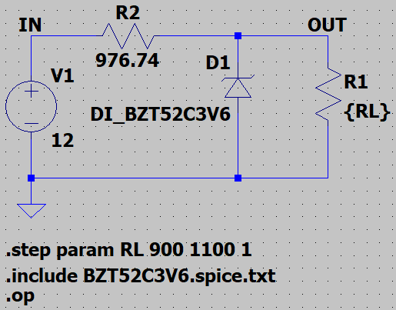
\includegraphics[width=\textwidth]{figures/loadreg_schem.png}
\end{column}
\begin{column}{0.3\textwidth}
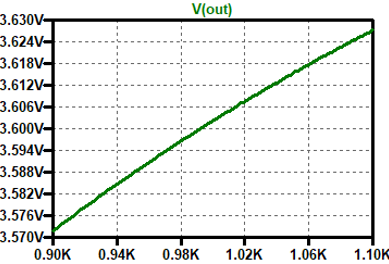
\includegraphics[width=\textwidth]{figures/loadreg_plot.png}
\end{column}
\begin{column}{0.3\textwidth}
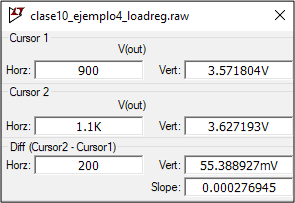
\includegraphics[width=\textwidth]{figures/loadreg_measure.png}

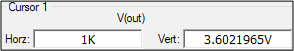
\includegraphics[width=\textwidth]{figures/loadreg_measure2.png}
\end{column}
\end{columns}

\[ LoadReg = \dfrac{3.627193 - 3.571804}{3.6021965} \times 100\% \]
\[ LoadReg = 1.54\% \]
\end{frame}


\section{Reguladores integrados}
\begin{frame}{El circuito integrado LM7805/7905}

\begin{itemize}
    \item El circuito integrado LM7805 entrega una tensión de salida constante de $+5\ V$.
    \item El complemento LM7905 entrega una tensión de salida negativa de $-5\ V$.
\end{itemize}

\begin{figure}
    \centering
    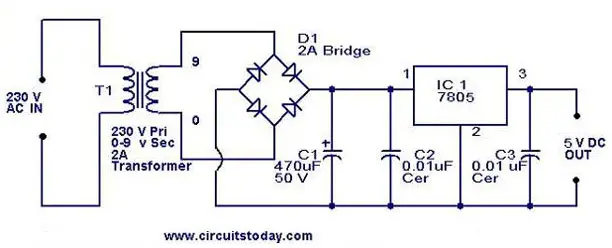
\includegraphics[width=0.8\textwidth]{figures/regulated_power_supply_1.png}
\end{figure}
\end{frame}


\begin{frame}{El circuito integrado LM317/337}

El regulador LM317 requiere de resistencias externas para ajustar la tensión de salida.

\begin{columns}
\begin{column}{0.6\textwidth}
\begin{figure}
    \centering
    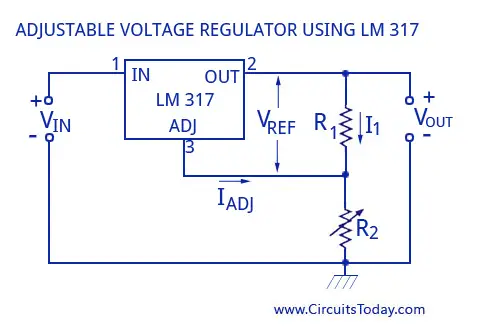
\includegraphics[width=\textwidth]{figures/lm317_working_principle.png}
\end{figure}
\end{column}
\begin{column}{0.4\textwidth}
\vspace{2mm}

La tensión de salida del LM317 se calcula con la ecuación:
%
\[ V_{out} = 1.25\ V \times \left( 1 + \dfrac{R_2}{R_1} \right) \]

Para el circuito complementario LM337 la tensión de salida es negativa:
%
\[ V_{out} = -1.25\ V \times \left( 1 + \dfrac{R_2}{R_1} \right) \]

\end{column}
\end{columns}
\end{frame}


\begin{frame}{El circuito integrado LM317/337}

Los circuitos integrados LM317/337 se pueden utilizar para construir una fuente regulada ajustable:

\begin{figure}
    \centering
    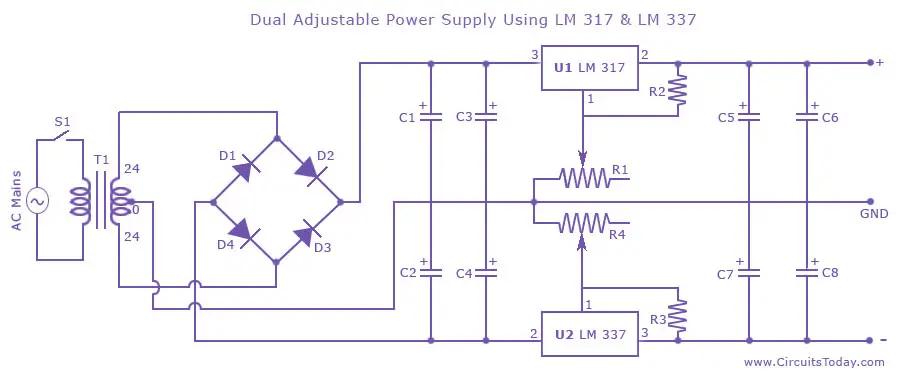
\includegraphics[width=0.8\textwidth]{figures/regulated_power_supply_2.png}
\end{figure}
\end{frame}


\section{Referencias}
\begin{frame}{Lecturas recomendadas}

\begin{itemize}
    \item Boylestad, R. y Nashelsky, L. (2009). Electrónica: Teoría de Circuitos y Dispositivos Electrónicos. Capítulo 2: Aplicaciones de los diodos, pp. 92-100, Pearson Educación, México.
    \item Razavi, B. (2013). Fundamentals of microelectronics, 2nd ed., pp. 99-105, Wiley, Los Angeles, California.
    \item Circuits Today (2023). 5V power supply using 7805. \url{https://www.circuitstoday.com/5v-power-supply-using-7805}
    \item Circuits Today (2023). Dual Adjustable Power Supply Using LM 317 \& LM337. \url{https://www.circuitstoday.com/dual-adjustable-power-supply-using-lm-317-lm337}
    \item Circuits Today (2023). IC Voltage Regulators. \url{https://www.circuitstoday.com/ic-voltage-regulators}
\end{itemize}

\end{frame}


\end{document}
